% Unit square and its image under T(x,y)=(2x+y,y). Area goes from 1 to |det T|=2.
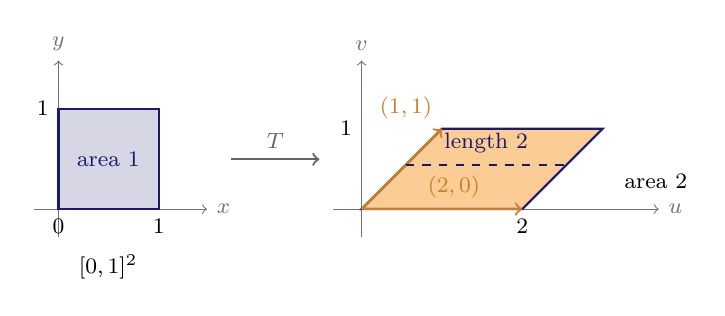
\begin{tikzpicture}[x=1.02cm,y=1.02cm,every node/.style={font=\footnotesize}]
  \draw[->,black!55] (-0.3,0) -- (1.85,0) node[right] {$x$};
  \draw[->,black!55] (0,-0.35) -- (0,1.85) node[above] {$y$};
  \fill[MidnightBlue!18] (0,0) rectangle (1.25,1.25);
  \draw[MidnightBlue,thick] (0,0) rectangle (1.25,1.25);
  \node[MidnightBlue] at (0.62,0.62) {area $1$};
  \node[below] at (0,0) {$0$};
  \node[below] at (1.25,0) {$1$};
  \node[left] at (0,1.25) {$1$};
  \node[anchor=north] at (0.62,-0.45) {$[0,1]^2$};
  \draw[->,thick,black!60] (2.15,0.62) -- (3.25,0.62) node[midway,above] {$T$};
  \begin{scope}[xshift=3.85cm]
    \draw[->,black!55] (-0.35,0) -- (3.7,0) node[right] {$u$};
    \draw[->,black!55] (0,-0.35) -- (0,1.85) node[above] {$v$};
    \fill[BurntOrange!38] (0,0) -- (2,0) -- (3,1) -- (1,1) -- cycle;
    \draw[MidnightBlue,thick] (0,0) -- (2,0) -- (3,1) -- (1,1) -- cycle;
    \draw[->,BurntOrange!80!black,thick] (0,0) -- (2,0);
    \draw[->,BurntOrange!80!black,thick] (0,0) -- (1,1);
    \node[BurntOrange!80!black,above] at (1.15,0.02) {$(2,0)$};
    \node[BurntOrange!80!black,above left] at (1,1) {$(1,1)$};
    \draw[MidnightBlue,thick,dashed] (0.55,0.55) -- (2.55,0.55);
    \node[MidnightBlue,anchor=south] at (1.55,0.58) {length $2$};
    \node[anchor=west] at (3.15,0.35) {area $2$};
    \node[below] at (2,0) {$2$};
    \node[left] at (0,1) {$1$};
  \end{scope}
\end{tikzpicture}
